\section{Implementation}
\label{sec:pumpkin-impl}

parts of PUMPKIN PATCH Inside the Core, plus more.

add something about Git, add something about hint application, add something about regrets (compiling to trees),
add something about optimization via the identity class of change.

\subsection{Tool Details}

% from Inside the Core
% Some of this may be better placed in earlier sections

While our system is a very early prototype under active development, we have made the source code available on Github.\footnote{\url{http://github.com/uwplse/PUMPKIN-PATCH/tree/cpp18}}
The interested reader can follow along in the repository. % This link is old, and it is no longer a prototype, so adjust
Our prototype has no impact on the trusted computing base (Section~\ref{sec:tcb}).

\subsubsection{Semantic Differencing} We implement semantic differencing over \emph{trees}:
\sysname compiles each proof term into a tree (\lstinline{evaluation.ml}). In these trees,
every node is a type context, and every edge is an extension to that type context with a 
new term.\footnote{These trees are inspired by categorical models of dependent type theory~\cite{Hofmann97}.}
Correspondingly, type differencing (to identify goal types) compares nodes, 
and term differencing (to find candidates) compares edges. 

The component (\lstinline{differencing.ml}) uses these nodes and edges to prioritize semantically
relevant differences. At the lowest level, it calls a primitive differencing function 
which checks if it can substitute one term within another term to find a function between their types.

The key benefit to this model is that it gives us a natural way to express inductive proofs, so
that differencing can efficiently identify good candidates.
Consider, for example, searching for a patch between conclusions of two inductive proofs of theorems about the natural numbers:

\begin{lstlisting}[language=coq]
  nat_ind (@\diff{P}@) ... (fun (IH : (@\diff{P}@) n) => ...) : (@\ltacforall@) n, (@\diff{P}@) n(@\vspace{-0.08cm}@)
  nat_ind (@\diff{P'}@) ... (fun (IH : (@\diff{P'}@) n) => ...) : (@\ltacforall@) n, (@\diff{P'}@) n
\end{lstlisting}
In each case, the component diffs the terms in the dotted edges of the tree for \lstinline{nat_ind} (Figure~\ref{fig:cattree}) to
try to find a term that maps between conclusions of that case:

\begin{lstlisting}[language=coq]
  P' (@\diff{0}@) -> P (@\diff{0}@)           (* base case candidate *)(@\vspace{-0.08cm}@)
  P' (@\diff{(S n)}@) -> P (@\diff{(S n)}@) (* inductive case candidate *)
\end{lstlisting}
The component also knows that the change in the type of \lstinline{IH} is inconsequential (it occurs for any change in conclusion).
Furthermore, it knows that \lstinline{IH} cannot show up as a hypothesis in the patch,
so it attempts to remove any occurrences of \lstinline{IH} in any candidate.

When the component finds a candidate, it knows \lstinline{P'} and \lstinline{P}
as well as the arguments \lstinline{0} or \lstinline{(S n)}. This makes it simple
to query abstraction for the final patch:

\begin{lstlisting}[language=coq]
  (@\ltacforall@) (@\diff{n}@), P' (@\diff{n}@) -> P (@\diff{n}@)
\end{lstlisting}
The differencing component is \textit{lazy}: it compiles terms into trees one step at a time.
It then \emph{expands} each tree as needed to find candidates (\lstinline{expansion.ml}).
For example, consider searching two functions for a patch between conclusions:
%For example, suppose both terms are functions that take an argument of the same type:

\begin{lstlisting}
  fun (t : T) => b(@\vspace{-0.08cm}@)
  fun (t' : T) => b'
\end{lstlisting}
Differencing introduces a single term of type \lstinline{T} to a common environment,
then expands and recursively diffs the bodies \lstinline{b} and \lstinline{b'} in that environment.

The tool always maintains pointers to easily switch between the tree and AST representations of the terms.
This representation enables extensibility.

\begin{figure}[t]
\begin{center}
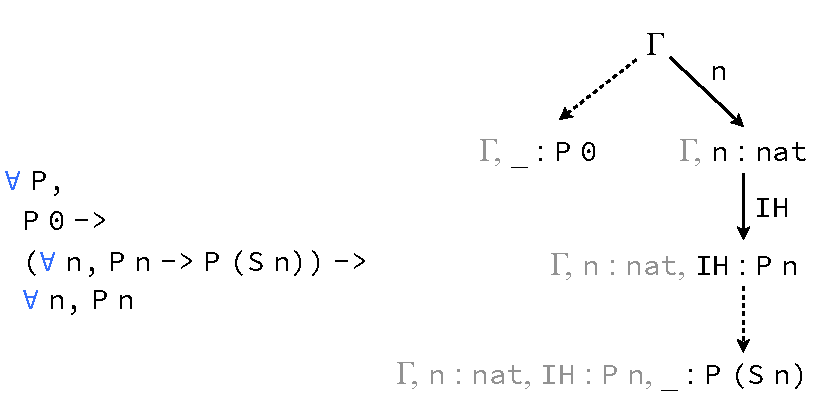
\includegraphics[scale=0.55]{repair/nat_ind}
\end{center}
\caption{The type of (left) and tree for (right) the induction principle \lstinline{nat_ind}. The solid edges represent hypotheses, and the dotted edges represent the proof obligations for each case in an inductive proof.}
\label{fig:cattree}
\end{figure}

\subsubsection{Transformations}

\paragraph{Patch Specialization} Specialization (\lstinline{specialize.ml}) takes a patch candidate and some arguments,
all of which are Coq terms.
It applies the candidate to the arguments, then it $\beta\iota$-reduces~\cite{equality} the result using Coq's
\lstinline{Reduction.nf_betaiota} function. It is the job of the 
patch finding procedure to provide both the candidate and the arguments.

\paragraph{Patch Abstraction} Abstraction (\lstinline{abstraction.ml}) takes a patch candidate, 
the goal type, and the function arguments or function to abstract.
It first generalizes the candidate, wrapping it inside of a lambda from the type of the term to abstract.
Then, it substitutes terms inside the body with the abstract term.
It continues to do this until there is nothing left to abstract, then filters results by the goal type.
Consider, for example, abstracting this candidate by \lstinline{m}:

\begin{lstlisting}[language=coq]
  fun (H : n <= m) => le_plus_trans n m 1 H(@\vspace{-0.04cm}@)
  : n <= m -> n <= m + 1
\end{lstlisting}
The generalization step wraps this in a lambda from some \lstinline{nat}, the type of \lstinline{m}:

\begin{lstlisting}[language=coq]
  fun ((@\diff{n0}@) : nat) =>(@\vspace{-0.04cm}@)
    (fun (H : n <= m) => le_plus_trans n m 1 H)(@\vspace{-0.04cm}@)
  : (@\ltacforall@) (@\diff{n0}@), n <= m -> n <= m + 1
\end{lstlisting}
The substitution step replaces \lstinline{m} with \lstinline{n0}:

\begin{lstlisting}[language=coq]
  fun ((@\diff{n0}@) : nat) =>(@\vspace{-0.04cm}@)
    (fun (H : n <= (@\diff{n0}@)) => le_plus_trans n (@\diff{n0}@) 1 H)(@\vspace{-0.04cm}@)
  : (@\ltacforall@) (@\diff{n0}@), n <= (@\diff{n0}@) -> n <= (@\diff{n0}@) + 1
\end{lstlisting}

Abstraction uses a list of \textit{abstraction strategies} to determine what subterms
to substitute. In this case, the simplest strategy works: The tool
replaces all terms that are convertible to the concrete argument \lstinline{m} with the abstract argument
\lstinline{n0}, which produces a single candidate. Type-checking this candidate confirms that it is a patch.

In some cases, the simplest strategy is not sufficient, even when it is possible to abstract the term.
It may be possible to produce a patch only by abstracting \emph{some} of the subterms
convertible to the argument or function (we show an example of this in Section~\ref{sec:fail}),
or the term may not contain any subterms convertible to the argument or function at all.
We implement several strategies to account for this. The combinations strategy, for example,
tries all combinations of substituting only some of the convertible subterms with the abstract argument. 
The pattern-based strategy substitutes subterms that match a certain pattern
with a term that corresponds to that pattern.

It is the job of the patch finding procedure to provide the candidate and the terms to abstract.
In addition, each configuration includes a list of strategies.
The configuration for changes in conclusions, for example, starts with the simplest strategy,
and moves on to more complex strategies only if that strategy fails.
This design makes abstraction simple to extend with new strategies and simple to call with different strategies
for different classes of changes.

\paragraph{Patch Inversion} Patch inversion (\lstinline{inverting.ml}) exploits symmetry to try to reverse the conclusions of a 
candidate patch.
It first factors the candidate using the factoring component, then calls the primitive inversion
function on each factor, then finally folds the resulting list in reverse.
The primitive inversion function exploits symmetry. 
For example, equality is symmetric, so the component can invert any application of \lstinline{eq_ind} or \lstinline{eq_ind_r}
(any rewrite). Indeed, \lstinline{eq_ind} and \lstinline{eq_ind_r} are inverses, and are related by symmetry:

\begin{lstlisting}[language=coq]
  (@\diff{eq\_ind\_r}@) A x P (H : P x) y (H0 : y = x) :=(@\vspace{-0.04cm}@)
    (@\diff{eq\_ind}@) x (fun y0 : A => P y0) H y ((@\diff{eq\_sym}@) H0)	
\end{lstlisting}
If inversion does not recognize that the type is symmetric, it
swaps subterms and type-checks the result to see if it is an inverse.

\paragraph{Lemma Factoring} The lemma factoring component (\lstinline{factoring.ml}) searches within a term
for its factors. For example,
if the term composes two functions, it returns both factors:

\begin{lstlisting}[language=coq]
  t : (@\diff{X}@) -> (@\diff{Z}@)                (* term *)(@\vspace{-0.04cm}@)
 [f : (@\diff{X}@) -> (@\diff{Y}@); g : (@\diff{Y}@) -> (@\diff{Z}@)] (* factors *)
\end{lstlisting}
In this case, the component takes the composite term and \lstinline{X} as arguments.
It first searches as deep as possible for a term of type \lstinline{X -> Y} for some \lstinline{Y}.
If it finds such a term, then it recursively searches for a term with type \lstinline{Y -> Z}. 
It maintains all possible 
paths of factors along the way, and it discards any paths that cannot reach \lstinline{Z}.

The current implementation can handle paths
with more than two factors, but it fails when \lstinline{Y} depends on \lstinline{X}.
Other components may benefit from dependent factoring; we leave this to future work.

\subsubsection{Inside the Procedure}
\label{sec:algimpl}

The implementation (\lstinline{patcher.ml4}) of the procedure from Section~\ref{sec:composeintro} starts with a
preprocessing step which compiles the proof terms to trees (like the tree in Figure~\ref{fig:cattree}).
It then searches for candidates one step at a time, expanding the trees when necessary.

The \sysname prototype exposes the patch finding procedure to users through the Coq 
command \lstinline{Patch Proof}. \sysname automatically
infers which configuration to use for the procedure from the example change. For example, to
find a patch for the case study in Section~\ref{sec:compcert}, we
used this command:

\begin{lstlisting}[language=ml4]
  Patch Proof Old.unsigned_range unsigned_range as patch.
\end{lstlisting}
\sysname analyzed both versions of \lstinline{unsigned_range} and determined 
that a constructor of the \lstinline{int} type changed (Figure~\ref{fig:int}),
so it initialized the configuration for changes in constructors.

Internally, \sysname represents configurations as sets of options,
which it passes to the procedure. The procedure uses these options to determine
how to compose components (for example, whether to abstract candidates) 
and how to customize components (for example, whether semantic differencing should look for an intermediate lemma).
To implement new configurations for different classes of changes, we simply tweak the options.

\subsection{Workflow Integration}

Needed: hints and so on, any work done since, the Git interface, whatever.

\subsubsection{Trusted Computing Base}
\label{sec:tcb}

A common concern for Coq plugins is an increase in the trusted computing base.
The Coq developers provide a safe plugin API in Coq 8.7 to address this~\cite{coq87news}.
Our prototype takes this into consideration:
While \sysname does not yet support Coq 8.7, it only calls the internal Coq functions that the 
developers plan to expose in the safe API~\cite{coqPR}.
Furthermore, Coq type-checks terms that plugins produce.
Since \sysname does not modify the type checker, it cannot produce an ill-typed term.
